\documentclass[reprint,amsmath,amssymb,aps]{revtex4-1}
\usepackage[spanish,es-tabla]{babel}
\usepackage[utf8]{inputenc}
\usepackage{graphicx}
\usepackage{dcolumn}
\usepackage{bm}
\usepackage{amsmath}
\usepackage{bigints}
\usepackage{gensymb}
\usepackage{mathrsfs}
\usepackage[T1]{fontenc}
\usepackage[none]{hyphenat}
\usepackage{booktabs}
\usepackage[normalem]{ulem}
\usepackage{soul}
\useunder{\uline}{\ul}{}
\usepackage[table,xcdraw]{xcolor}
\usepackage{newunicodechar}
\usepackage{enumerate}
\usepackage{hyperref}
\renewcommand\thesection{\arabic{section}}
\renewcommand{\tablename}{TABLA}
%\newunicodechar{°}{\degree}
\usepackage{float}
\usepackage{etoolbox}
\usepackage{dirtytalk}
\spanishdecimal{.}
\makeatletter
\patchcmd{\frontmatter@RRAP@format}{(}{}{}{}
\patchcmd{\frontmatter@RRAP@format}{)}{}{}{}
\renewcommand\Dated@name{}
\makeatother


\begin{document}
\footnotesize
\preprint{APS/123-QED}

\title{Proyecto Astrofísica Computacional 2}

\author{\large Eduardo Andrés Delgadillo Monsalve, Iván Gabriel Mafla Bolaños, Nicola Sebastián Miranda Niño}
 \affiliation{\texttt{eadelgadillom@unal.edu.co,}\texttt{imafla@unal.edu.co,}\texttt{nsmirandan@unal.edu.co}\\
 \normalsize { Universidad Nacional de Colombia, Sede Bogotá. 3 de Diciembre del 2023}
 }
\begin{abstract}
\normalsize
\begin{center}\textbf{Resumen}\\
\end{center}
Este proyecto se centró en la resolución numérica de la ecuación de Poisson en el contexto del modelo de Plummer, un problema relevante en astrofísica computacional. El objetivo fue calcular el potencial gravitacional \(\Phi(x, y, z)\) para una distribución de masa esférica descrita por el modelo de Plummer. Para abordar este problema, se implementó inicialmente el método de diferencias finitas en coordenadas cartesianas. Esta aproximación transformó la ecuación de Poisson, \(\nabla^2 \Phi = 4\pi G\rho\), en un sistema de ecuaciones algebraicas sobre una malla bidimensional, en primer lugar, y luego en una tridimensional. Se aplicaron dos métodos iterativos para resolver este sistema: el método de Jacobi y el método de Gauss-Seidel. Ambos métodos se basan en la actualización iterativa de los valores del potencial en cada punto de la malla, utilizando los valores de los puntos vecinos. Mientras que en el método de Jacobi se utilizaron los valores de la iteración anterior para todas las actualizaciones, en el método de Gauss-Seidel se empleó una mezcla de valores antiguos y nuevos, lo que llevó a una convergencia más rápida. Con el método de Jacobi, se observó una convergencia lenta y problemas de estabilidad. El método de Gauss-Seidel, aunque potencialmente más eficiente, enfrentó desafíos similares y complicaciones adicionales relacionadas con la implementación computacional. El desarrollo del proyecto muestra las dificultades inherentes a la aplicación de métodos numéricos en problemas complejos de astrofísica. El análisis realizado proporciona una base importante para futuras investigaciones y sugiere la necesidad de explorar técnicas alternativas o ajustes adicionales para resolver eficazmente la ecuación de Poisson en el contexto de astrofísica computacional.
 
\textbf{Palabras Clave: } Ecuación de Poisson, Modelo de Plummer, Algoritmo de Jacobi, Algoritmo de Gauss-Seidel, Diferencias Finitas. 
\end{abstract}
\maketitle

\section{Introducción}
El problema planteado en el proyecto consiste en aplicar el método de diferencias finitas para resolver una ecuación de Poisson, donde la densidad de masa está dada por el modelo de Plummer. La ecuación de Poisson es una ecuación diferencial parcial fundamental en la física y la astrofísica. Es una generalización de la ley de Gauss del campo gravitacional y describe cómo un campo gravitacional es afectado por una distribución de masa presente. 

La ecuación de Poisson que relaciona el potencial gravitacional $\Phi(x)$ con la densidad de masa se expresa como 
\begin{equation}
    \nabla^2 \Phi = 4 \pi G \rho
\end{equation}
En coordenadas cartesianas el operador Laplaciano se expresa como
\begin{equation}
    \nabla^2 = \frac{\partial^2}{\partial x^2} + \frac{\partial^2}{\partial y^2} + \frac{\partial^2}{\partial z^2}
\end{equation}
La densidad de masa $\rho(r)$ en el modelo de Plummer es \cite{plummer}:
\begin{equation}\label{plummer}
\rho(r) = \frac{3M_0}{4\pi a^3} \left( 1 + \frac{r^2}{a^2} \right)^{-\frac{5}{2}}
\end{equation}
Aquí, $M_0$ alude a la masa del cúmulo y $a$ es un parámetro conocido como el radio de Plummer. El modelo de Plummer es un modelo simplificado que se utiliza para describir la distribución de masa en sistemas astronómicos, como cúmulos estelares. Esta fórmula implica que la densidad disminuye con la distancia desde el centro del cúmulo, pero nunca llega a cero, aproximándose a un comportamiento tipo ley de potencia para grandes distancias \cite{poissonGauss}.

En el proyecto se implementa un código en Python para resolver la ecuación de Poisson y compara los resultados obtenidos con los resultados analíticos donde
\begin{equation}
\varPhi=-\frac{GM_{0}}{\sqrt{r^2+a^2}},
\end{equation}
para evaluar la exactitud del método. También se aplica algún algoritmo de relajación como el método de Jacobi y el de Gauss-Seidel.

La solución se centra en implementar el método de diferencias finitas para la ecuación de Poisson en un sistema cartesiano y calcular el potencial gravitacional para la esfera de Plummer.

\section{Marco Teórico}
Se realiza la implementación del método de diferencias finitas en Python para resolver la ecuación de Poisson con la densidad de masa dada por el modelo de Plummer \cite{laplacian}. Para el caso 2D, el código crea una grilla bidimensional y calcula el potencial gravitacional $\Phi(x,y)$ en cada punto de esta grilla.

El ajuste y precisión de la implementación dependen de las condiciones del problema, en función de las cuales se deben ajustar los parámetros como el tamaño de la grilla, las dimensiones físicas de la grilla, y los valores específicos de $M_0$ y $a$.

Además, en el proyecto se extiende el método a un dominio tridimensional, implementando técnicas de relajación como el método de Jacobi \cite{jacobi} y el de Gauss-Seidel \cite{poissonGauss}. En este caso, los resultados se presentan con secciones transversales (un plano bidimensional) del potencial gravitacional, las cuales representan un plano que corta la esfera de Plummer, mostrando la variación del potencial.

Para visualizar el potencial en una esfera de Plummer, se calcula el potencial en puntos distribuidos uniformemente en el volumen de la esfera que permitan manejar correctamente la geometría esférica.

\subsection{Método de diferencias finitas en 2D y 3D}
Se utilizó el método de diferencias finitas para aproximar numéricamente la solución de la ecuación de Poisson para el modelo de Plummer. Se implementó una versión 2D y luego se extendió a 3D \cite{fdm}.

Para la implementación en Python se definió una grilla 2D y una 3D para el cálculo del potencial gravitacional. En 3D, la grilla se extiende a lo largo de tres ejes espaciales utilizando coordenadas cartesianas (ejes x, y, z). Aunque el problema es esencialmente esférico, las coordenadas cartesianas se utilizaron para simplificar la implementación del método de diferencias finitas \cite{laplacian}.

La densidad en el modelo de Plummer se describe naturalmente en términos de la distancia radial (cantidad esférica), sin embargo, esta distancia se calculó a partir de las coordenadas cartesianas de cada punto en la grilla. La distancia radial $r$ se calcula utilizando la relación
\begin{equation}
    r = \sqrt{x^2 + y^2 + z^2}
\end{equation}
El método de diferencias finitas se aplicó en el dominio cartesiano, actualizando los valores del potencial en cada punto de la grilla basándose en los valores de sus vecinos inmediatos, lo que es más directo en un sistema cartesiano.

Luego, se usa la fórmula de densidad de Plummer para calcular la densidad de masa en cada punto de la grilla. Se aplicó el método de diferencias finitas y en el caso de 3D, los algoritmos de relajación mencionados para resolver la ecuación de Poisson en la grilla.

En los códigos desarrollados, el Laplaciano se utiliza implícitamente en el proceso de resolver la ecuación de Poisson utilizando el método de diferencias finitas. El Laplaciano se calcula como la suma de las diferencias entre el valor del potencial en ese punto y los valores en los puntos vecinos, dividido por el cuadrado del tamaño del paso de la grilla dx, dy y dz en coordenadas cartesianas\cite{laplacian}.

En el modelo 2D el Laplaciano se calcula como
\begin{equation}\label{Laplaciano2D}
\begin{split}
\nabla^2 \Phi \approx & \frac{\Phi(i+1, j) + \Phi(i-1, j)}{\Delta x^2} \\
& + \frac{\Phi(i, j+1) + \Phi(i, j-1) - 4\Phi(i, j)}{\Delta x^2}
\end{split}
\end{equation}
y se utiliza para actualizar el valor del potencial en cada iteración del algoritmo.
De esta ecuación es posible encontrar la ecuación iterativa de diferencias finitas, como un sistema lineal de ecuaciones de la forma:
\begin{equation}
    \mathcal{M} \Phi = R
    \label{kan:1}
\end{equation}

Donde $M$ es la matriz o grilla de dimensiones definida, entonces a partir de (\ref{Laplaciano2D}) se tiene que:

\begin{equation}
\begin{split}
    \Phi(x_{i+1},y_i)  + \Phi(x_{i-1},y_i) +\\ \Phi(x_i,y_{i+1})  + \Phi(x_i,y_{i-1}) - \\ 4\Phi(x_i,y_i) =  h^2 \rho (x_i,y_i)
\end{split}
\end{equation}
Esto, escrito de forma matricial se puede representar como:
\begin{equation}\label{matriz}
\begin{pmatrix}
-4 & 1 & 0 & 1 & 0 & \dots \\ 
1 & -4 & 1 & 0 & 0 & \dots \\
0 & 1 & -4 & 1 & 0 & \dots \\
1 & 0 & 1 & -4 & 0 & \dots \\
\vdots & \vdots & \vdots & \vdots & \vdots & 
\end{pmatrix}
\begin{pmatrix}
\phi_{0,0}\\ \phi_{1,0} \\ \phi_{2,0} \\ \vdots \\ \phi_{M,N}
\end{pmatrix}=
\begin{pmatrix}
R_1 \\
\vdots\\
\vdots\\
R_n
\end{pmatrix}
\end{equation}

Para el caso de 3 dimensiones se procede de manera similar, en donde son 3 las componentes totales del sistema, por lo que el sistema lineal de ecuaciones puede ser resuelto al definir una matriz de dimensión $N^3 \times N^3$, donde $N$ es la cantidad de puntos sobre los ejes de la grilla, en caso de que estén separados igualmente separados. \cite{Seidel}.


\subsection{Método de Jacobi y Metodo Gauss-Seidel}

Se realizó una extensión del problema para ser resuelto tridimensionalmente, para eso se utilizaron los denominados métodos de relajación. Estos métodos son útiles para resolver sistemas de ecuaciones lineales como es el caso de \ref{kan:1}. Se basan principalmente en acercarse a la solución de manera iterativa por medio del ajuste de una solución hasta alcanzar la convergencia. Por lo general, se comienza el proceso con un ansatz inicial (forma de una solución tentativa) y luego se modifica con bucles o iteraciones hasta encontrar la solución verdadera.
Si bien los métodos de Jacobi y Gauss-Seidel son parecidos difieren en pequeñas cosas, especialmente en como actualizan las soluciones de cada iteración, esto hace que el método de Jacobi sea más sencillo de implementar, pero el de Gauss-Seidel sea mas óptimo lo que logra mejorar el tiempo de cálculo debido a que converge más rápido a la solución \cite{poissonGauss, jacobi}.

En resumen ambos métodos se pueden resumir como \cite{laplacian}:
\begin{enumerate}
    \item Se inicializa la matriz $\phi_{i,j}$ con un ansatz inicial
    \item Se aplican las condiciones de frontera o condiciones iniciales
     \item En el modelo 3D el Laplaciano se calcula como la cantidad:
    \begin{equation}
    \begin{split}
    \nabla^2 \Phi \approx \, & \frac{\Phi(i+1, j, k) + \Phi(i-1, j, k)}{\Delta x^2} + \\
                         & \frac{\Phi(i, j+1, k) + \Phi(i, j-1, k)}{\Delta x^2} + \\
                         & \frac{\Phi(i, j, k+1) + \Phi(i, j, k-1) - 6\Phi(i, j, k)}{\Delta x^2}
    \end{split}
    \end{equation}
    Este cálculo se usa para actualizar el valor del potencial en cada punto de la grilla tridimensional en cada iteración del algoritmo de Jacobi y de Gauss-Seidel
    \item Para el método de Jacobi,en cada punto interior se reemplaza $\phi_{i,j}$ por $\phi^*_{i,j}$ donde:
    \begin{equation}\label{Jacobi}
    \begin{split}
    \Phi_{i,j,k}^{(n+1)} = \frac{1}{6} \Bigl( \Phi_{i+1,j,k}^{(n)} + \Phi_{i-1,j,k}^{(n)} + \\
    \Phi_{i,j+1,k}^{(n)} + \Phi_{i,j-1,k}^{(n)} + \\ \Phi_{i,j,k+1}^{(n)} + \Phi_{i,j,k-1}^{(n)} - h^2 \pi G \rho_{i,j,k} \Bigr)
    \end{split}
    \end{equation}

    \item Para el método de Gauss-Seidel el remplazo de $\phi_{i,j}$ por $\phi^*_{i,j}$ se hace directamente en la ecuación del punto 3, es decir:
    \begin{equation}\label{Gauss}
    \begin{split}
        \Phi_{i,j,k}^{(n+1)} = \frac{1}{6} \Bigl( \Phi_{i+1,j,k}^{(n+1)} + \Phi_{i-1,j,k}^{(n)} + \\
    \Phi_{i,j+1,k}^{(n+1)} + \Phi_{i,j-1,k}^{(n)} + \\ \Phi_{i,j,k+1}^{(n+1)} + \Phi_{i,j,k-1}^{(n)} - h^2 \pi G \rho_{i,j,k} \Bigr)
    \end{split}
    \end{equation}
    
    \item Se vuelve al paso 2 hasta que la diferencia entre las dos aproximaciones mas recientes sea más pequeña que una tolerancia predeterminada.
\end{enumerate}

En la implementación 2D, el término $-4\Phi(i, j)$ no se usa explícitamente. En su lugar, el nuevo valor del potencial en cada punto se calcula promediando sus valores en los puntos vecinos y sumando el término relacionado con la densidad de masa $4\pi G \rho(i, j) \cdot dx \cdot dy$. Esto es equivalente a incluir implícitamente el término mencionado en el cálculo del Laplaciano.

En la implementación 3D con el método de Jacobi, el término $-6\Phi(i, j, k)$ tampoco aparece explícitamente. Al igual que en el caso 2D, el nuevo valor del potencial en cada punto se determina promediando los valores en los puntos vecinos y sumando el término de densidad. La ausencia explícita de este término es una característica del método de Jacobi, donde el valor actual del punto no se resta explícitamente, ya que se utiliza una copia anterior de la matriz de potencial para calcular los nuevos valores.

\subsection{Aplicación en Astrofísica}
Un caso de aplicación de la ecuación de Poisson y el modelo de Plummer en astrofísica es en el estudio y modelado de cúmulos estelares \cite{astro,astro1,astro2}. Los cúmulos estelares son agrupaciones de estrellas que pueden proporcionar información valiosa sobre la formación y evolución de las galaxias. Al aplicar el modelo de Plummer, se puede obtener la siguiente información:
\begin{itemize}
    \item Estimar la distribución de masa dentro del cúmulo.
     \item Analizar la dinámica de las estrellas y el comportamiento
    \item Entender cómo la distribución de masa afecta las trayectorias y velocidades de las estrellas en el cúmulo.
\end{itemize}

Este modelo también es la base para modelos más complejos que pueden incluir, por ejemplo, efectos como la elipticidad del cúmulo, la rotación, y la presencia de materia oscura. Además, proporciona el fundamento teórico para la simulación numérica y la visualización de cúmulos estelares en estudios astrofísicos.

\section{Implementación y Resultados}
Para solucionar la ecuación de Poisson asociada con el potencial gravitacional con una densidad de la esfera de Plummer, inicialmente se implementó el método de las diferencias finitas, en el lenguaje de programación Python, para el caso 2D con una función de densidad sencilla que se puede escribir como
\begin{equation}
    \rho(x,y)=-2\pi \sin(\pi x) \sin (\pi y)
\end{equation}
en una región del espacio cuadrada con límites en $x=[0,1]$ y $y=[0,1]$ donde las condiciones de frontera están dadas por
\begin{eqnarray}
&\varPhi(0,y)=0 \label{asu:1}\\
&\varPhi(1,y)=0 \label{asu:2}\\
&\varPhi(x,0)=0 \label{asu:3}\\
&\varPhi(x,1)=0 \label{asu:4}
\end{eqnarray}
lo cual implica que la solución analítica de este problema será 
\begin{equation}
\varPhi(x,y)=\sin(\pi x) \sin (\pi y) \label{asu:5}
\end{equation}
por lo que de esta forma se tiene una referencia para comparar los resultados numéricos que brinde el código.\\

Así que para implementar el método inicialmente se creó una función denominada \texttt{InicializarMatriz2D} la cual inicializa una matriz de dimensión $N^2 \times  N^2$, donde $N$ representa el número de intervalos en que se dividió cada eje, que se caracteriza por el hecho de que todas las filas asociadas a la frontera toman un valor de $1$ en la diagonal y $0$ en los demás elementos, mientras que para los nodos toma la forma que representa el sistema de ecuaciones lineales dada por el método de las diferencias finitas (\ref{matriz}).

Posteriormente, se implementa la función \texttt{densidad} donde se introduce el valor de $\rho(x,y)$. En la función \texttt{condicionesdefrontera2D} se diseña el vector $b$ del sistema de ecuaciones donde se asigna el valor a los elementos de la frontera que están dados por las ecuaciones \ref{asu:1}, \ref{asu:2}, \ref{asu:3} y \ref{asu:4}. \\

Ahora bien, para resolver este sistema de ecuaciones se diseñaron tres funciones, a saber:
\begin{itemize}
    \item \texttt{solverInv}: Con esta función se resuelve el sistema de ecuaciones al calcular la inversa de la matriz mediante la función \texttt{linalg.solve} de la librería Numpy.
    \item \texttt{solverJacobi}: En esta función se implementa el método de Jacobi para resolver el sistema de ecuaciones de interés.
    \item \texttt{GaussSeidelSolver}: Con esta función se utiliza el método de Gauss-Seidel para resolver el sistema de ecuaciones de interés.
\end{itemize}
En las Figuras \ref{fig:1}, \ref{fig:2} y \ref{fig:3} (que se pueden apreciar mejor en el código adjunto a este documento) se ilustran los resultados de cada uno de estos métodos, para el caso de $N=100$, y se comparan con el resultado analítico. Así mismo, en la tabla \ref{tab:1} se presenta el error cuadrático medio de cada uno de estos métodos.\\
\begin{figure}
    \centering
    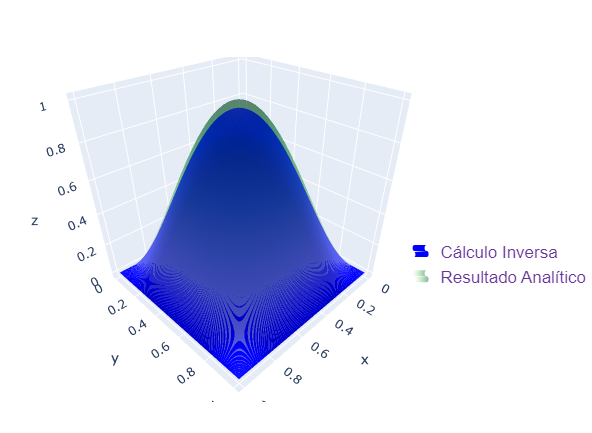
\includegraphics[width=0.5\textwidth]{2dinv.png}
    \caption{Potencial gravitacional $\varPhi$, localizado en el eje Z con unidades $M_{\odot} ua^2/yr^2$, respecto a las coordenadas en $x$ y $y$ en unidades astronómicas. Nótese que se compara el resultado obtenido analíticamente con el resultado obtenido al calcular directamente la inversa de la matriz.}
    \label{fig:1}
\end{figure}
\begin{figure}
    \centering
    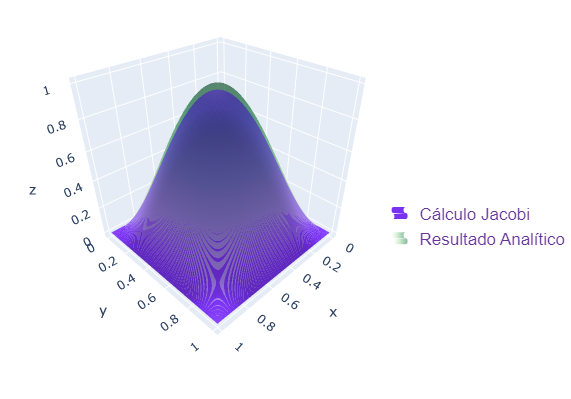
\includegraphics[width=0.5\textwidth]{2djacobi.png}
    \caption{Potencial gravitacional $\varPhi$, localizado en el eje Z con unidades $M_{\odot} ua^2/yr^2$, respecto a las coordenadas en $x$ y $y$ en unidades astronómicas. Nótese que se compara el resultado obtenido analíticamente con el resultado obtenido mediante el método de Jacobi.}
    \label{fig:2}
\end{figure}
\begin{figure}
    \centering
    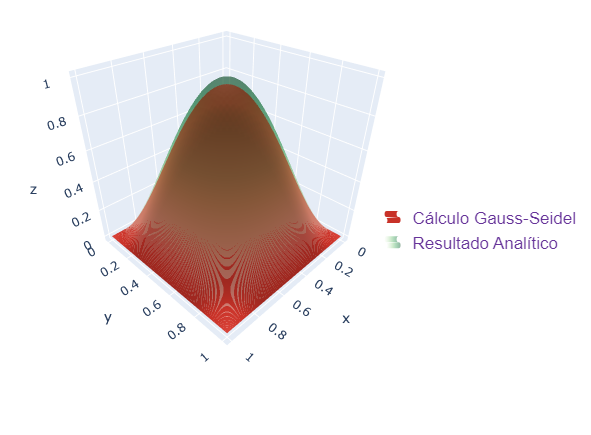
\includegraphics[width=0.5\textwidth]{2dgauss.png}
    \caption{Potencial gravitacional $\varPhi$, localizado en el eje Z con unidades $M_{\odot} ua^2/yr^2$, respecto a las coordenadas en $x$ y $y$ en unidades astronómicas. Nótese que se compara el resultado obtenido analíticamente con el resultado obtenido mediante el método de Gauss-Seidel.}
    \label{fig:3}
\end{figure}
\begin{table}
    \centering
    \begin{tabular}{|c|c|} \hline
    \rowcolor[HTML]{EFEFEF}
         Método & Error Cuadrático Medio \\ \hline
         Inversa Directa &  0.000370 \\ \hline
         Jacobi & 0.000370\\ \hline
         Gauss-Seidel & 0.000374\\ \hline
    \end{tabular}
    \caption{Error cuadrático medio obtenido al comparar los resultados numéricos de cada método con el resultado analítico para el caso 2D.}
    \label{tab:1}
\end{table}
Una vez implementado el código en dos dimensiones se procede de manera similar para el caso de tres dimensiones, donde se crea un conjunto de funciones, análogo al caso de bidimensional, que se describen a continuación:
\begin{itemize}
    \item \texttt{InicializarMatriz3D}: Mediante esta función se crea una matriz que representa el sistema de ecuaciones planteado por el método de las diferencias finitas (\ref{matriz}) pero en este caso se introduce mediante el producto de Kronecker. Asimismo, en las filas que corresponden a los nodos de la frontera se le da valor de $0$ a todos lo elementos menos a los de la diagonal que toman un valor de $1$.
    \item \texttt{densidad3D}: En esta función se implementa la densidad de materia $\rho(x,y,z)$.
    \item \texttt{condicionesdefrontera3D}: En esta función se crea el vector $\textbf{b}$ que contiene el valor del término $4\pi \rho(x,y,z)$ de cada nodo y de las condiciones de frontera.
    \item \texttt{solverInv3D}: Al igual que en el caso 2D se resuelve el sistema calculando directamente la inversa de la matriz mediante el uso de la función \texttt{linalg.solve} de la libreria Numpy.
    \item \texttt{solverJacobi}: Se implementa el método de Jacobi para solucionar el sistema de ecuaciones.
    \item \texttt{GaussSeidelSolver3D}: Mediante esta función se implementa el método de Gauss-Seidel para resolver el sistema de ecuaciones de interés.
\end{itemize}
Ahora bien, la densidad de masa de la esfera de Plummer se encuentra dada por (\ref{plummer}) y las condiciones de frontera en un cubo delimitado en las regiones $x=[-0.5,0.5]$, $y=[-0.5,0.5]$ y $z=[-0.5,0.5]$ y en el que $M=1 M_{\odot}$ y $a=1 \hspace{0.1 cm} ua$ estarán dadas por
\begin{eqnarray}
    \varPhi(-0.5,y,z)= \frac{3}{4\pi} \left( 1.25+y^2+z^2 \right)^{-\frac{5}{2}}\\
    \varPhi(0.5,y,z)= \frac{3}{4\pi} \left( 1.25+y^2+z^2 \right)^{-\frac{5}{2}}\\
    \varPhi(x,-0.5,z)=\frac{3}{4\pi} \left( 1.25+x^2+z^2 \right)^{-\frac{5}{2}}\\
    \varPhi(x,0.5,z)=\frac{3}{4\pi} \left( 1.25+x^2+z^2 \right)^{-\frac{5}{2}}\\\\
    \varPhi(x,y,-0.5)=\frac{3}{4\pi} \left( 1.25+x^2+y^2 \right)^{-\frac{5}{2}}\\
    \varPhi(x,y,0.5)=\frac{3}{4\pi} \left( 1.25+x^2+y^2 \right)^{-\frac{5}{2}}.
\end{eqnarray}
Así que, al resolver el sistema de ecuaciones con $N=25$, mediante los diferentes métodos descritos previamente, se obtienen los cortes del potencial gravitacional asociado a la Esfera de Plummer, los cuales se ilustran en las Figuras \ref{fig:4}, \ref{fig:5} y \ref{fig:6} (que se pueden apreciar de mejor manera en el código adjunto a este documento). Además, en la tabla \ref{tab:2} se presenta el error cuadrático medio que se obtuvo para cada uno de los métodos utilizados para obtener el potencial. \\
\begin{figure}
    \centering
    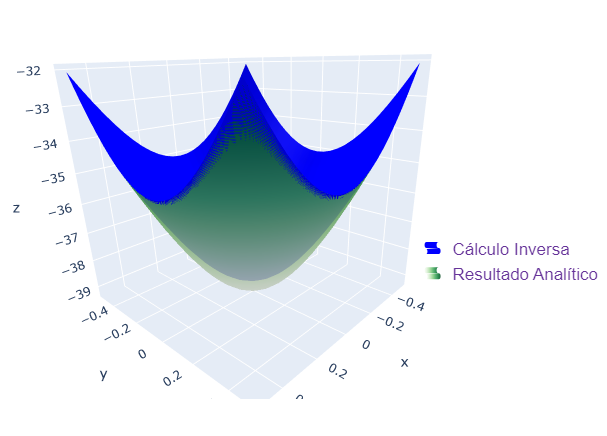
\includegraphics[width=0.5\textwidth]{3dinv.png}
    \caption{Representación de una sección transversal en $z=-0.125 \hspace{0.1 cm} ua$ del potencial gravitacional $\varPhi$, cuyo valor se localiza en el eje Z con unidades $M_{\odot} ua^2/yr^2$, respecto a las coordenadas en $x$ y $y$ que se encuentran en unidades astronómicas. Nótese que se compara el resultado obtenido analíticamente con el resultado obtenido al calcular directamente la inversa de la matriz.}
    \label{fig:4}
\end{figure}
\begin{figure}
    \centering
    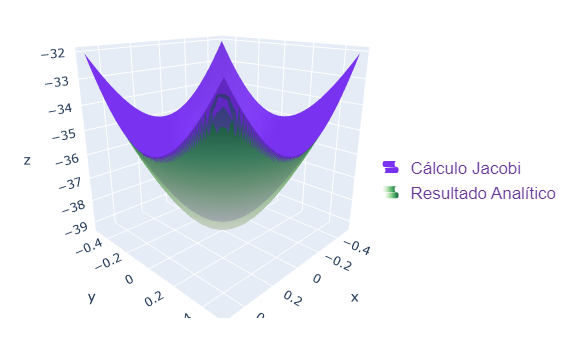
\includegraphics[width=0.5\textwidth]{3djacobi.png}
    \caption{Representación de una sección transversal en $z=-0.125 \hspace{0.1 cm} ua$ del potencial gravitacional $\varPhi$, cuyo valor se localiza en el eje Z con unidades $M_{\odot} ua^2/yr^2$, respecto a las coordenadas en $x$ y $y$ que se encuentran en unidades astronómicas. Nótese que se compara el resultado obtenido analíticamente con el resultado obtenido mediante el método de Jacobi.}
    \label{fig:5}
\end{figure}
\begin{figure}
    \centering
    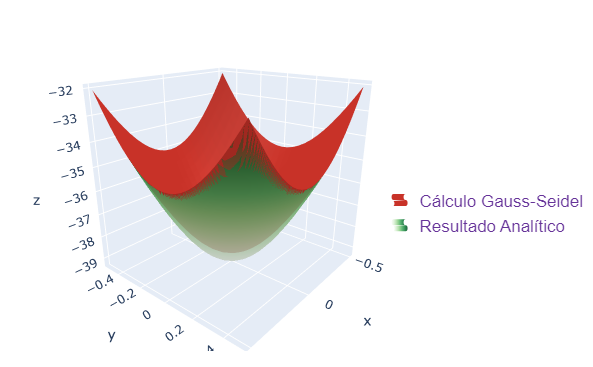
\includegraphics[width=0.5\textwidth]{3dgauss.png}
    \caption{Representación de una sección transversal en $z=-0.125 \hspace{0.1 cm} ua$ del potencial gravitacional $\varPhi$, cuyo valor se localiza en el eje Z con unidades $M_{\odot} ua^2/yr^2$, respecto a las coordenadas en $x$ y $y$ que se encuentran en unidades astronómicas. Nótese que se compara el resultado obtenido analíticamente con el resultado obtenido mediante el método de Gauss-Seidel.}
    \label{fig:6}
\end{figure}
\begin{table}
    \centering
    \begin{tabular}{|c|c|} \hline
    \rowcolor[HTML]{EFEFEF}
         Método & Error Cuadrático Medio \\ \hline
         Inversa Directa &   0.02472 \\ \hline
         Jacobi & 0.02473\\ \hline
         Gauss-Seidel & 0.02472\\ \hline
    \end{tabular}
    \caption{Error cuadrático medio obtenido al comparar los resultados numéricos de cada método con el resultado analítico para el caso 3D.}
    \label{tab:2}
\end{table}

Nótese que en las figuras \ref{fig:4}, \ref{fig:5} y \ref{fig:6}, se aprecia el comportamiento esperado para el potencial gravitacional, ya que esta cantidad toma un mayor valor absoluto en proximidad al origen puesto que en dicha región se encuentra una mayor concentración de masa que en los bordes.\\

Por último, es relevante destacar que el método de diferencias finitas permite resolver adecuadamente el problema del potencial gravitacional dado por la ecuación de Poisson. Sin embargo, al aumentar el valor de $N$ el cálculo directo de la inversa de la matriz se vuelve más costoso computacionalmente hasta el punto que el código dejaba de correr. Por esta razón, se implementaron los métodos de Jacobi y Gauss-Seidel, que permitían realizar el cálculo para mayores valores de $N$, donde se destaca que el tiempo de convergencia es menor para el algoritmo de Gauss-Seidel en relación al de Jacobi.\\

 
\section{Conclusiones}
Las visualizaciones en 2D muestran imágenes con cortes transversales del potencial, revelando cómo el potencial gravitacional varía con la distancia desde el centro. Estas visualizaciones son útiles para entender la simetría y la distribución del potencial en secciones planas.

La representación en 3D proporciona una visión integral de la distribución del potencial en la esfera de Plummer. El potencial es más alto cerca del centro y disminuye hacia el exterior, lo cual es coherente con las expectativas teóricas del modelo de Plummer.

Los códigos implementados presentan un enfoque numérico para resolver la ecuación de Poisson en el contexto de la esfera de Plummer, y las visualizaciones proporcionan una comprensión profunda de la naturaleza tridimensional del potencial gravitacional en un marco astrofísico.

El uso de coordenadas cartesianas en problemas con geometría esférica puede presentar ciertas limitaciones en términos de precisión y eficiencia, especialmente cerca del centro o en regiones con simetría esférica. Sin embargo, para el desarrollo del proyecto, las coordenadas cartesianas permitieron una implementación más sencilla y directa del método de diferencias finitas y facilitaron la visualización y la comprensión del problema.

El método de Jacobi puede ser lento para converger, especialmente para mallas grandes. Por esto, es importante elegir un tamaño de paso adecuado para garantizar la estabilidad del método. Aunque el método de Jacobi es inherentemente paralelizable, se requiere cuidado en la implementación para garantizar la eficiencia.

El método de Gauss-Seidel puede converger más rápido que el método de Jacobi, especialmente para matrices que son diagonalmente dominantes. La convergencia y la velocidad del método pueden depender de la elección de los valores iniciales. A diferencia del método de Jacobi, la paralelización del método de Gauss-Seidel es menos directa debido a su naturaleza secuencial en la actualización de los valores.

Como alternativa al método de diferencias finitas, existe el método de elementos finitos (FEM), que se puede aplicar utilizando herramientas especializadas como FEniCS. El FEM, con su capacidad para manejar dominios complejos y condiciones de frontera, puede presentarse como una opción viable para abordar las limitaciones encontradas en el proyecto.

\bibliographystyle{plain}
\bibliography{biblio}

\end{document}
